\documentclass[tikz,border=0pt]{standalone}
\usepackage{xcolor}
% Palette: Sam_Comm_final.png by eye (as Pursuer's art.py), and Gatecrasher's own.
\definecolor{ink}{HTML}{3B2340}
\definecolor{sky}{HTML}{EFC46A}
\definecolor{skyhi}{HTML}{F5DA92}
\definecolor{skylow}{HTML}{E9B060}
\definecolor{cloud}{HTML}{F2D58A}
\definecolor{wallA}{HTML}{E88A73}
\definecolor{wallB}{HTML}{EE9F7E}
\definecolor{wallC}{HTML}{E47A7E}
\definecolor{wallD}{HTML}{F0B07E}
\definecolor{wallE}{HTML}{D9765F}
\definecolor{wallF}{HTML}{E99A8A}
\definecolor{greenA}{HTML}{8DBB7E}
\definecolor{greenB}{HTML}{6FA77A}
\definecolor{greenC}{HTML}{A9C97F}
\definecolor{greenD}{HTML}{5E9C6A}
\definecolor{window}{HTML}{F6E7A0}
\definecolor{windark}{HTML}{8C5A64}
\definecolor{metal}{HTML}{8D9A93}
\definecolor{metaldark}{HTML}{5E6B66}
\definecolor{wood}{HTML}{B9835A}
\definecolor{paving}{HTML}{E2BD8C}
\definecolor{ground}{HTML}{D3A77D}
\definecolor{stone}{HTML}{E7C9A0}
\definecolor{paper}{HTML}{F6E7C4}
\definecolor{cardboard}{HTML}{C9A06A}
\definecolor{cardboarddark}{HTML}{A47C4C}
\definecolor{red}{HTML}{B3262E}
\definecolor{eyewhite}{HTML}{FBF4E4}
\definecolor{skin}{HTML}{E8B07C}
\definecolor{skinB}{HTML}{C98B5E}
\definecolor{skinC}{HTML}{F2C9A0}
\definecolor{hairdark}{HTML}{2A1E33}
\definecolor{hairred}{HTML}{A8553A}
\definecolor{leather}{HTML}{33293D}
\definecolor{chrome}{HTML}{C9D3CF}
\definecolor{chromedark}{HTML}{7F8C88}
\definecolor{glass}{HTML}{A9D4CB}
\definecolor{lamp}{HTML}{FFE6A3}
\definecolor{smoke}{HTML}{E8D3AE}
\definecolor{shingle}{HTML}{C9604F}
\definecolor{gold}{HTML}{F2B53A}
\definecolor{portalblue}{HTML}{2FA8E8}
\definecolor{portalbluehi}{HTML}{A6DDF5}
\definecolor{portalorange}{HTML}{F2812E}
\definecolor{portalorangehi}{HTML}{F9C891}
\definecolor{olive}{HTML}{7A8450}
\definecolor{olivedark}{HTML}{5C6539}
\definecolor{khaki}{HTML}{C2A66E}
\definecolor{khakidark}{HTML}{9E8350}
\definecolor{mule}{HTML}{9A6A44}
\definecolor{muledark}{HTML}{6B4730}
\definecolor{mulelight}{HTML}{C99A6E}
\definecolor{bandana}{HTML}{C8343A}
\definecolor{suit}{HTML}{56704F}
\definecolor{camoA}{HTML}{8DA867}
\definecolor{camoB}{HTML}{3B5240}
\definecolor{lens}{HTML}{8EF0C6}
\definecolor{lenshi}{HTML}{E2FFF2}
\definecolor{sea}{HTML}{5FB3B0}
\definecolor{seahi}{HTML}{8FCFC0}
\definecolor{seadark}{HTML}{3F8F92}
\definecolor{concrete}{HTML}{E6C29A}
\definecolor{concretedark}{HTML}{C9A07A}
\definecolor{heli}{HTML}{4F8F86}
\definecolor{helidark}{HTML}{3A6C66}
\definecolor{duskA}{HTML}{7A5272}
\definecolor{duskB}{HTML}{B06A78}
\definecolor{duskC}{HTML}{DE8E72}
\definecolor{dirt}{HTML}{C08A68}
\definecolor{dirtdark}{HTML}{A87256}
\definecolor{beam}{HTML}{FFF3BE}
\definecolor{sunA}{HTML}{F3B86A}
\definecolor{sunB}{HTML}{EE9268}
\definecolor{sunC}{HTML}{E57766}
\definecolor{sundisc}{HTML}{FBE3A0}
\definecolor{seadusk}{HTML}{6F9E9C}
\definecolor{balloon}{HTML}{F8F0DE}
\definecolor{hay}{HTML}{E9C46A}
\definecolor{haydark}{HTML}{C99B45}
\definecolor{barn}{HTML}{C9604F}
\definecolor{trim}{HTML}{F6E7C4}
\begin{document}
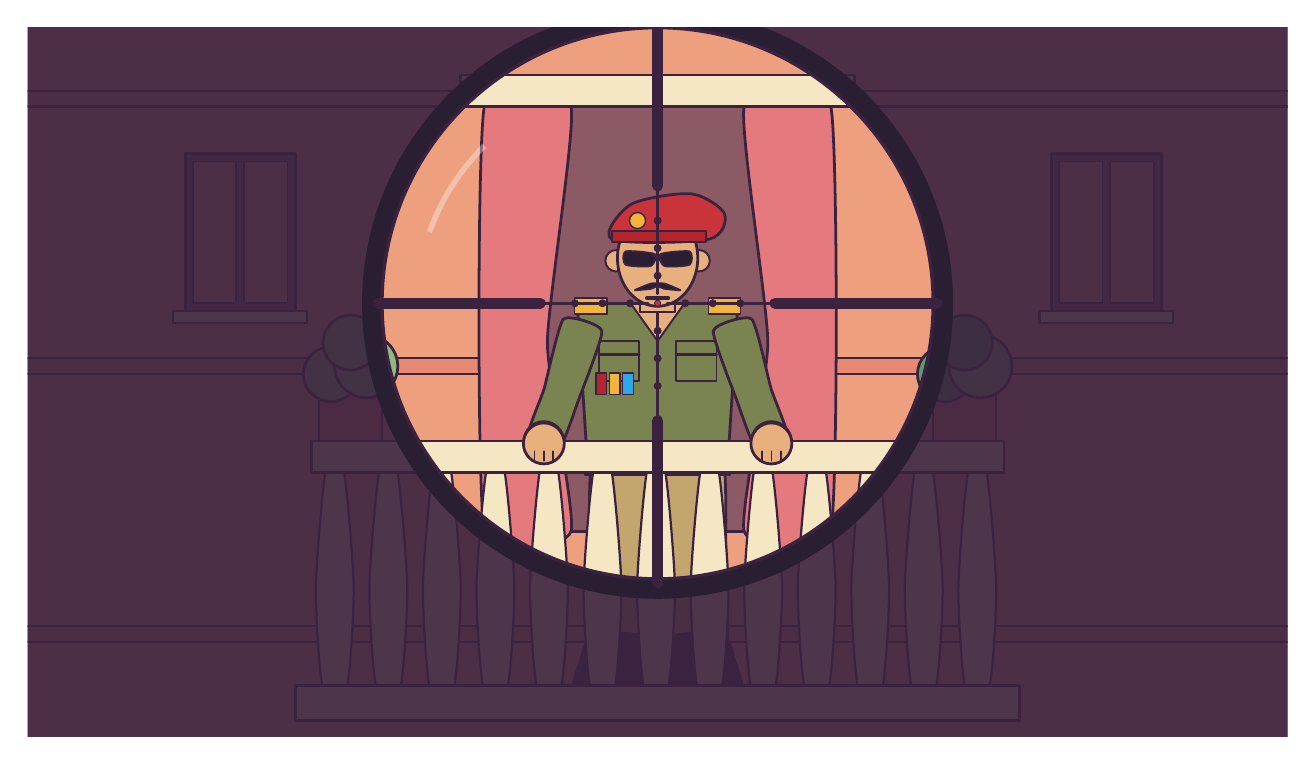
\begin{tikzpicture}
\useasboundingbox (0,0) rectangle (16,9);
\clip (0,0) rectangle (16,9);
\filldraw[draw=ink, line width=1pt, line join=round, fill=wallB] (-0.2,-0.2) -- (16.2,-0.2) -- (16.2,9.2) -- (-0.2,9.2) -- cycle;
\filldraw[draw=ink, line width=0.8pt, line join=round, fill=wallA] (-0.2,1.2) -- (16.2,1.2) -- (16.2,1.4) -- (-0.2,1.4) -- cycle;
\filldraw[draw=ink, line width=0.8pt, line join=round, fill=wallA] (-0.2,4.6) -- (16.2,4.6) -- (16.2,4.8) -- (-0.2,4.8) -- cycle;
\filldraw[draw=ink, line width=0.8pt, line join=round, fill=wallA] (-0.2,8) -- (16.2,8) -- (16.2,8.2) -- (-0.2,8.2) -- cycle;
\filldraw[draw=ink, line width=1pt, line join=round, fill=windark] (2,5.4) -- (3.4,5.4) -- (3.4,7.4) -- (2,7.4) -- cycle;
\filldraw[draw=ink, line width=0.8pt, line join=round, fill=trim] (1.85,5.25) -- (3.55,5.25) -- (3.55,5.4) -- (1.85,5.4) -- cycle;
\filldraw[draw=ink, line width=0.7pt, line join=round, fill=wallF] (2.1,5.5) -- (2.65,5.5) -- (2.65,7.3) -- (2.1,7.3) -- cycle;
\filldraw[draw=ink, line width=0.7pt, line join=round, fill=wallF] (2.75,5.5) -- (3.3,5.5) -- (3.3,7.3) -- (2.75,7.3) -- cycle;
\filldraw[draw=ink, line width=1pt, line join=round, fill=windark] (13,5.4) -- (14.4,5.4) -- (14.4,7.4) -- (13,7.4) -- cycle;
\filldraw[draw=ink, line width=0.8pt, line join=round, fill=trim] (12.85,5.25) -- (14.55,5.25) -- (14.55,5.4) -- (12.85,5.4) -- cycle;
\filldraw[draw=ink, line width=0.7pt, line join=round, fill=wallF] (13.1,5.5) -- (13.65,5.5) -- (13.65,7.3) -- (13.1,7.3) -- cycle;
\filldraw[draw=ink, line width=0.7pt, line join=round, fill=wallF] (13.75,5.5) -- (14.3,5.5) -- (14.3,7.3) -- (13.75,7.3) -- cycle;
\filldraw[draw=ink, line width=1pt, line join=round, fill=windark] (5.8,2.6) -- (10.2,2.6) -- (10.2,8) -- (5.8,8) -- cycle;
\filldraw[draw=ink, line width=1pt, line join=round, fill=wallC] plot[smooth cycle, tension=0.3] coordinates {(5.8,8) (6.9,8) (6.6,5) (6.9,2.6) (5.8,2.6)};
\filldraw[draw=ink, line width=1pt, line join=round, fill=wallC] plot[smooth cycle, tension=0.3] coordinates {(10.2,8) (9.1,8) (9.4,5) (9.1,2.6) (10.2,2.6)};
\filldraw[draw=ink, line width=1pt, line join=round, fill=trim] (5.5,8) -- (10.5,8) -- (10.5,8.4) -- (5.5,8.4) -- cycle;
\filldraw[draw=ink, line width=1pt, line join=round, fill=khaki] plot[smooth cycle, tension=0.3] coordinates {(7.999,3.544) (7.846,2.196) (7.779,1.066) (7.133,1.086) (7.134,2.234) (7.185,3.606)};
\filldraw[draw=ink, line width=1pt, line join=round, fill=leather] plot[smooth cycle, tension=0.25] coordinates {(7.83,0.6) (6.946,0.6) (7.014,0.94) (7.15,1.28) (7.762,1.28)};
\draw[khakidark, line width=1.36pt, line cap=round, line join=round] (7.49,2.725) -- (7.49,2.045);
\filldraw[draw=ink, line width=1pt, line join=round, fill=khaki] plot[smooth cycle, tension=0.3] coordinates {(8.815,3.606) (8.866,2.234) (8.867,1.086) (8.221,1.066) (8.154,2.196) (8.001,3.544)};
\filldraw[draw=ink, line width=1pt, line join=round, fill=leather] plot[smooth cycle, tension=0.25] coordinates {(8.17,0.6) (9.054,0.6) (8.986,0.94) (8.85,1.28) (8.238,1.28)};
\draw[khakidark, line width=1.36pt, line cap=round, line join=round] (8.51,2.725) -- (8.51,2.045);
\filldraw[draw=ink, line width=1pt, line join=round, fill=olive] (7.116,3.354) -- (8.884,3.354) -- (9.02,5.496) -- (6.98,5.496) -- cycle;
\filldraw[draw=ink, line width=0.8pt, line join=round, fill=leather] (7.082,3.32) -- (8.918,3.32) -- (8.918,3.626) -- (7.082,3.626) -- cycle;
\filldraw[draw=ink, line width=0.6pt, line join=round, fill=gold] (7.83,3.32) -- (8.17,3.32) -- (8.17,3.626) -- (7.83,3.626) -- cycle;
\filldraw[draw=ink, line width=0.7pt, line join=round, fill=olive] (7.762,4.51) -- (7.252,4.51) -- (7.252,5.02) -- (7.762,5.02) -- cycle;
\draw[ink, line width=1.02pt, line cap=round, line join=round] (7.762,4.85) -- (7.252,4.85);
\filldraw[draw=ink, line width=0.7pt, line join=round, fill=olive] (8.238,4.51) -- (8.748,4.51) -- (8.748,5.02) -- (8.238,5.02) -- cycle;
\draw[ink, line width=1.02pt, line cap=round, line join=round] (8.238,4.85) -- (8.748,4.85);
\filldraw[draw=ink, line width=0.7pt, line join=round, fill=skin] (7.66,5.496) -- (8,5.02) -- (8.34,5.496) -- cycle;
\draw[ink, line width=1.19pt, line cap=round, line join=round] (8,5.02) -- (8,3.66);
\filldraw[draw=ink, line width=0.6pt, line join=round, fill=gold] (7.354,5.36) -- (6.946,5.36) -- (6.946,5.564) -- (7.354,5.564) -- cycle;
\filldraw[draw=ink, line width=0.6pt, line join=round, fill=gold] (8.646,5.36) -- (9.054,5.36) -- (9.054,5.564) -- (8.646,5.564) -- cycle;
\filldraw[draw=ink, line width=0.5pt, line join=round, fill=red] (7.218,4.34) -- (7.354,4.34) -- (7.354,4.612) -- (7.218,4.612) -- cycle;
\filldraw[draw=ink, line width=0.5pt, line join=round, fill=gold] (7.388,4.34) -- (7.524,4.34) -- (7.524,4.612) -- (7.388,4.612) -- cycle;
\filldraw[draw=ink, line width=0.5pt, line join=round, fill=portalblue] (7.558,4.34) -- (7.694,4.34) -- (7.694,4.612) -- (7.558,4.612) -- cycle;
\filldraw[draw=ink, line width=1pt, line join=round, fill=olive] plot[smooth cycle, tension=0.3] coordinates {(7.292,5.149) (6.994,4.267) (6.754,3.671) (6.356,3.819) (6.558,4.413) (6.804,5.299)};
\filldraw[draw=ink, line width=0.8pt, line join=round, fill=skin] (6.555,3.745) circle (0.255);
\filldraw[draw=ink, line width=1pt, line join=round, fill=olive] plot[smooth cycle, tension=0.3] coordinates {(9.196,5.299) (9.442,4.413) (9.644,3.819) (9.246,3.671) (9.006,4.267) (8.708,5.149)};
\filldraw[draw=ink, line width=0.8pt, line join=round, fill=skin] (9.445,3.745) circle (0.255);
\filldraw[draw=ink, line width=0.7pt, line join=round, fill=skin] (7.779,5.394) -- (8.221,5.394) -- (8.221,5.666) -- (7.779,5.666) -- cycle;
\filldraw[draw=ink, line width=0.7pt, line join=round, fill=skin] (7.473,6.04) circle (0.136);
\filldraw[draw=ink, line width=0.7pt, line join=round, fill=skin] (8.527,6.04) circle (0.136);
\filldraw[draw=ink, line width=1pt, line join=round, fill=skin] plot[smooth cycle, tension=0.55] coordinates {(8.51,6.074) (8.493,6.232) (8.442,6.38) (8.361,6.507) (8.255,6.604) (8.132,6.665) (8,6.686) (7.868,6.665) (7.745,6.604) (7.639,6.507) (7.558,6.38) (7.507,6.232) (7.49,6.074) (7.507,5.916) (7.558,5.768) (7.639,5.641) (7.745,5.544) (7.868,5.483) (8,5.462) (8.132,5.483) (8.255,5.544) (8.361,5.641) (8.442,5.768) (8.493,5.916)};
\filldraw[draw=ink, line width=0.6pt, line join=round, fill=hairdark] plot[smooth cycle, tension=0.4] coordinates {(7.966,6.125) (7.592,6.159) (7.592,5.989) (7.915,5.972)};
\filldraw[draw=ink, line width=0.6pt, line join=round, fill=hairdark] plot[smooth cycle, tension=0.4] coordinates {(8.034,6.125) (8.408,6.159) (8.408,5.989) (8.085,5.972)};
\draw[ink, line width=1.36pt, line cap=round, line join=round] (7.949,6.108) -- (8.051,6.108);
\filldraw[draw=ink, line width=0.6pt, line join=round, fill=hairdark] plot[smooth cycle, tension=0.3] coordinates {(7.711,5.666) (7.915,5.751) (8.085,5.751) (8.289,5.666) (8.085,5.683) (8,5.717) (7.915,5.683)};
\draw[ink, line width=1.36pt, line cap=round, line join=round] (7.864,5.564) -- (8.136,5.564);
\filldraw[draw=ink, line width=1pt, line join=round, fill=bandana] plot[smooth cycle, tension=0.5] coordinates {(7.422,6.312) (7.66,6.754) (8.425,6.89) (8.85,6.635) (8.646,6.312)};
\filldraw[draw=ink, line width=0.6pt, line join=round, fill=red] (7.422,6.278) -- (8.612,6.278) -- (8.612,6.414) -- (7.422,6.414) -- cycle;
\filldraw[draw=ink, line width=0.5pt, line join=round, fill=gold] (7.745,6.55) circle (0.102);
\filldraw[draw=ink, line width=0.8pt, line join=round, fill=paper] plot[smooth cycle, tension=0.4] coordinates {(3.75,0.6) (4.05,0.6) (4.14,1.9) (4.01,3.4) (3.79,3.4) (3.66,1.9)};
\filldraw[draw=ink, line width=0.8pt, line join=round, fill=paper] plot[smooth cycle, tension=0.4] coordinates {(4.43,0.6) (4.73,0.6) (4.82,1.9) (4.69,3.4) (4.47,3.4) (4.34,1.9)};
\filldraw[draw=ink, line width=0.8pt, line join=round, fill=paper] plot[smooth cycle, tension=0.4] coordinates {(5.11,0.6) (5.41,0.6) (5.5,1.9) (5.37,3.4) (5.15,3.4) (5.02,1.9)};
\filldraw[draw=ink, line width=0.8pt, line join=round, fill=paper] plot[smooth cycle, tension=0.4] coordinates {(5.79,0.6) (6.09,0.6) (6.18,1.9) (6.05,3.4) (5.83,3.4) (5.7,1.9)};
\filldraw[draw=ink, line width=0.8pt, line join=round, fill=paper] plot[smooth cycle, tension=0.4] coordinates {(6.47,0.6) (6.77,0.6) (6.86,1.9) (6.73,3.4) (6.51,3.4) (6.38,1.9)};
\filldraw[draw=ink, line width=0.8pt, line join=round, fill=paper] plot[smooth cycle, tension=0.4] coordinates {(7.15,0.6) (7.45,0.6) (7.54,1.9) (7.41,3.4) (7.19,3.4) (7.06,1.9)};
\filldraw[draw=ink, line width=0.8pt, line join=round, fill=paper] plot[smooth cycle, tension=0.4] coordinates {(7.83,0.6) (8.13,0.6) (8.22,1.9) (8.09,3.4) (7.87,3.4) (7.74,1.9)};
\filldraw[draw=ink, line width=0.8pt, line join=round, fill=paper] plot[smooth cycle, tension=0.4] coordinates {(8.51,0.6) (8.81,0.6) (8.9,1.9) (8.77,3.4) (8.55,3.4) (8.42,1.9)};
\filldraw[draw=ink, line width=0.8pt, line join=round, fill=paper] plot[smooth cycle, tension=0.4] coordinates {(9.19,0.6) (9.49,0.6) (9.58,1.9) (9.45,3.4) (9.23,3.4) (9.1,1.9)};
\filldraw[draw=ink, line width=0.8pt, line join=round, fill=paper] plot[smooth cycle, tension=0.4] coordinates {(9.87,0.6) (10.17,0.6) (10.26,1.9) (10.13,3.4) (9.91,3.4) (9.78,1.9)};
\filldraw[draw=ink, line width=0.8pt, line join=round, fill=paper] plot[smooth cycle, tension=0.4] coordinates {(10.55,0.6) (10.85,0.6) (10.94,1.9) (10.81,3.4) (10.59,3.4) (10.46,1.9)};
\filldraw[draw=ink, line width=0.8pt, line join=round, fill=paper] plot[smooth cycle, tension=0.4] coordinates {(11.23,0.6) (11.53,0.6) (11.62,1.9) (11.49,3.4) (11.27,3.4) (11.14,1.9)};
\filldraw[draw=ink, line width=0.8pt, line join=round, fill=paper] plot[smooth cycle, tension=0.4] coordinates {(11.91,0.6) (12.21,0.6) (12.3,1.9) (12.17,3.4) (11.95,3.4) (11.82,1.9)};
\filldraw[draw=ink, line width=1pt, line join=round, fill=trim] (3.6,3.35) -- (12.4,3.35) -- (12.4,3.75) -- (3.6,3.75) -- cycle;
\filldraw[draw=ink, line width=1pt, line join=round, fill=trim] (3.4,0.2) -- (12.6,0.2) -- (12.6,0.65) -- (3.4,0.65) -- cycle;
\filldraw[draw=ink, line width=1pt, line join=round, fill=skin] (6.555,3.72) circle (0.26);
\draw[ink, line width=0.6pt, line cap=round, line join=round] (6.435,3.5) -- (6.435,3.62);
\draw[ink, line width=0.6pt, line cap=round, line join=round] (6.555,3.5) -- (6.555,3.62);
\draw[ink, line width=0.6pt, line cap=round, line join=round] (6.675,3.5) -- (6.675,3.62);
\filldraw[draw=ink, line width=1pt, line join=round, fill=skin] (9.445,3.72) circle (0.26);
\draw[ink, line width=0.6pt, line cap=round, line join=round] (9.325,3.5) -- (9.325,3.62);
\draw[ink, line width=0.6pt, line cap=round, line join=round] (9.445,3.5) -- (9.445,3.62);
\draw[ink, line width=0.6pt, line cap=round, line join=round] (9.565,3.5) -- (9.565,3.62);
\filldraw[draw=ink, line width=0.8pt, line join=round, fill=wallE] (3.7,3.75) -- (4.5,3.75) -- (4.5,4.35) -- (3.7,4.35) -- cycle;
\filldraw[draw=ink, line width=1pt, line join=round, fill=greenA] (3.85,4.6) circle (0.35);
\filldraw[draw=ink, line width=1pt, line join=round, fill=greenA] (4.3,4.7) circle (0.4);
\filldraw[draw=ink, line width=1pt, line join=round, fill=greenA] (4.1,5) circle (0.35);
\filldraw[draw=ink, line width=0.8pt, line join=round, fill=wallE] (11.5,3.75) -- (12.3,3.75) -- (12.3,4.35) -- (11.5,4.35) -- cycle;
\filldraw[draw=ink, line width=1pt, line join=round, fill=greenD] (11.65,4.6) circle (0.35);
\filldraw[draw=ink, line width=1pt, line join=round, fill=greenA] (12.1,4.7) circle (0.4);
\filldraw[draw=ink, line width=1pt, line join=round, fill=greenD] (11.9,5) circle (0.35);
\fill[ink, fill opacity=0.9, even odd rule] (-0.2,-0.2) rectangle (16.2,9.2) (8,5.5) circle (3.55);
\draw[hairdark, line width=7pt] (8,5.5) circle (3.63);
\draw[ink, line width=1.2pt] (8,5.5) circle (3.5);
\draw[ink, line width=4pt, line cap=round, line join=round] (4.45,5.5) -- (6.509,5.5);
\draw[ink, line width=4pt, line cap=round, line join=round] (8,1.95) -- (8,4.009);
\draw[ink, line width=1pt, line cap=round, line join=round] (6.509,5.5) -- (7.88,5.5);
\draw[ink, line width=1pt, line cap=round, line join=round] (8,4.009) -- (8,5.38);
\filldraw[draw=ink, line width=0.3pt, line join=round, fill=ink] (7.65,5.5) circle (0.045);
\filldraw[draw=ink, line width=0.3pt, line join=round, fill=ink] (8,5.15) circle (0.045);
\filldraw[draw=ink, line width=0.3pt, line join=round, fill=ink] (7.3,5.5) circle (0.045);
\filldraw[draw=ink, line width=0.3pt, line join=round, fill=ink] (8,4.8) circle (0.045);
\filldraw[draw=ink, line width=0.3pt, line join=round, fill=ink] (6.95,5.5) circle (0.045);
\filldraw[draw=ink, line width=0.3pt, line join=round, fill=ink] (8,4.45) circle (0.045);
\draw[ink, line width=4pt, line cap=round, line join=round] (11.55,5.5) -- (9.491,5.5);
\draw[ink, line width=4pt, line cap=round, line join=round] (8,9.05) -- (8,6.991);
\draw[ink, line width=1pt, line cap=round, line join=round] (9.491,5.5) -- (8.12,5.5);
\draw[ink, line width=1pt, line cap=round, line join=round] (8,6.991) -- (8,5.62);
\filldraw[draw=ink, line width=0.3pt, line join=round, fill=ink] (8.35,5.5) circle (0.045);
\filldraw[draw=ink, line width=0.3pt, line join=round, fill=ink] (8,5.85) circle (0.045);
\filldraw[draw=ink, line width=0.3pt, line join=round, fill=ink] (8.7,5.5) circle (0.045);
\filldraw[draw=ink, line width=0.3pt, line join=round, fill=ink] (8,6.2) circle (0.045);
\filldraw[draw=ink, line width=0.3pt, line join=round, fill=ink] (9.05,5.5) circle (0.045);
\filldraw[draw=ink, line width=0.3pt, line join=round, fill=ink] (8,6.55) circle (0.045);
\filldraw[draw=ink, line width=0.3pt, line join=round, fill=bandana] (8,5.5) circle (0.04);
\draw[white, line width=2pt, opacity=0.35] (5.8,7.5) arc (135:160:3);
\end{tikzpicture}
\end{document}
